\documentclass[12pt]{amsart}

\usepackage{dsfont}
\usepackage{amsmath}
\usepackage{amssymb}
\usepackage{extarrows}
\usepackage{color}
\usepackage{tcolorbox}
\tcbuselibrary{skins}
\definecolor{hellgrau}{gray}{.7}

\usepackage{amsrefs}

\renewcommand {\H}{H}
\newcommand{\C}{\mathcal{C}}
\newcommand{\Ab}{\mathbf{Ab}}


\begin{document}
\title{Methods of Homological
Algebra}

\begin{abstract}
This is a collection of
summaries of talks given in an 
undergraduate learning
seminar. Each talk is based on 
one section in Gelfan'd and
Manin's book on homological
algebra, and the summaries are
written by the speakers
themselves.
\end{abstract}
\maketitle

\tableofcontents 

\include{ha-ws20-uli}
\include{ha-ws20-andre}
\include{ha-ws20-tim}
\include{ha-ws20-anke}
\include{ha-ws20-josefin}
\include{ha-ws20-jasmin}
\include{ha-ws20-paula}
\documentclass[12pt]{article}
\usepackage{graphicx}

\begin{document}

\title{Derived Categories and Localisation}
\author{Sascha Roggatz}
\maketitle
\tableofcontents
\newpage

\section{Grundlagen}
\subsection{Wichtige Begriffe zu Kategorien}

Betrachte folgendes Setting\\
- C, D Kategorien, $F : C \mapsto D$ Funktor, $B \subset C$, $a,b,s,q,x,z \in Obj(C)$, $f : a \mapsto b$ \\
\newline
Dann heisst\\
- B  vollstaendige Unterkategorie von C, falls
\begin{description}
    \item[i) $Obj(B) \subset Obj(C)$]
    \item[ii) $\forall X,Y \in Obj(B): Mor_B(X,Y) = Mor_C(X,Y)$]  
\end{description}
- Morphismus $m : a \mapsto b$ monomorph, falls
\begin{description}
    \item[i) $fuer \: g_1,g_2 : x \mapsto a \: folgt \: aus \: m \circ g_1 = m \circ g_2 \Rightarrow g_1 = g_2$] 
\end{description}
- Morphismus $e : a \mapsto b$ epimorph, falls
\begin{description}
    \item[i) $fuer \: g_1,g_2 : b \mapsto x \: folgt \: aus \: g_1 \circ e = g_2 \circ e \Rightarrow g_1 = g_2$] 
\end{description}
- Morphismus $k : d \mapsto a$ Kern, falls
\begin{description}
    \item[i) $f \circ k = 0$]
    \item[ii) $zu \: h : x \mapsto a \: \exists ! h' : x \mapsto d: h = k \circ h'$] 
\end{description}
- Morphismus $k : b \mapsto d$ Kokern, falls
\begin{description}
    \item[i) $k \circ f = 0$]
    \item[ii) $zu \: h : b \mapsto x \: \exists ! h' : d \mapsto x: h = h' \circ k$] 
\end{description}
- Funktor F  volltreu, falls 
\begin{description}
    \item[i) $Mor_C(a,b) \mapsto Mor_D(F(a),F(b)), f \mapsto F(f) \: bijektiv$] 
\end{description}
- Funktor F  Aequivalenz von kategorien, falls
\begin{description}
    \item[i) $\exists G : D \mapsto C, \: sodass \: F \circ G \cong id_D \: und \: G \circ F \cong id_C$] 
\end{description}

\subsection{Was ist eine abelsche Kategorie?}

Sei A Kategorie. A heisst abelsch, falls $\forall X,Y,Z \in$ Obj(A):
\begin{description}
    \item[i) $\forall f,f_1,f_2 \in Hom_A(X,Y), g,g_1,g_2 \in Hom_A(Y,Z):$]
        \[g \circ (f_1 + f_2) = g \circ f_1 + g \circ f_2\]
        \[(g_1 + g_2) \circ f = g_1 \circ f + g_2 \circ f\]
    \item[ii) $\forall X_1,X_2 \exists X_1 \otimes X_2 \: mit \: Morphismen \: p_v : X_1 \otimes X_2 \mapsto X_v \: und \: i_v : X_i \mapsto X_1 \otimes X_2:$]
        \[p_v \circ i_v = id_{X_v}\]
        \[i_1 \circ p_1 + i_2 \circ p_2 = id_{X_1 \otimes X_2}\]
    \item[iii) $\exists \: Nullobjekte$]
    \item[iv) $\exists \: Kerne,\: Kokerne$]
    \item[v) $Jeder \: Monomorphismus \: ist \: Kern, \: jeder \: Epimorphismus \: ist \: Kokern$]   
\end{description}
    
\subsection{Was sind Kettenkomplexe?}

Eine Familie $C_n$ von Objekten aus abelschen Kategorie mit Morphismen $d_n : C_n \mapsto C_{n-1}$, sodass $d_n \circ d_{n+1} : C_{n+1} \mapsto C_{n-1} = 0$ 
heisst Kettenkomplex. Dazu definieren wir $H_n(C) := ker(d_n) / im(d_{n+1})$ und bezeichnen dieses als Homologieobjekt. Ein Kettenkomplex $(C_*, d_*)$ 
heisst exakt, falls alle $H_n(C)$ verschwinden. Wir nennen $Kom(A)$ die Kategorie der Kettenkomplexe abelscher Kategorien. Ein Morphismus $u : C \mapsto D$ 
von Kettenkomplexen ist eine Familie von Morphsimen $u_n : C_n \mapsto D_n$. $u: C \mapsto D$ heisst quasi-Isomorphismus, falls alle 
$H_n(C) \mapsto H_n(D)$ Isomorphismen sind.
\newpage

\section{Abgeleitete Kategorien}
\subsection{Definition}

Sei A abelsche Kategorie und Kom(A) die Kategorie der Komplexe über A.
Dann $\exists$ Kategorie D(A) und ein Funktor $Q: Kom(A) \mapsto D(A):$
\begin{description}
    \item[i) $Q(f) \: ist \: Isomorphismus \: fuer \: jeden \: quasi-Isomorphismus \: f: A \mapsto B$:]
        \[H_n(A_0) \mapsto H_n(B_0) \: ist \: Isomorphismus\]
    \item[ii) $Fuer \: jeden \: Funktor \: F : Kom(A) \mapsto D \: gilt$:]
        \[\exists! Funktor \: G : D(A) \mapsto D: F = G \circ D\]
\end{description}
D(A) heisst abgeleitete Kategorie von A. A heisst halbeinfach, falls jedes exakte Triple
T in A isomorph zu $0 \mapsto X \mapsto X \oplus Y \mapsto Y \mapsto 0$ ist. 

\subsection{Beweisskizze zur Existenz eine Lokalisierung}

Sei B eine Kategorie und S eine Klasse von Morphismen in B. Wir wollen eine Kategorie $B[S^{-1}] =: B_S$ und einen 
Funktor $Q : B \mapsto B_S$ konstruieren. Dazu setzen wir $Obj(B_S) = Obj(B)$ und gehen wir folgt vor:\\
- Konstruiere Morphismen in $B_S$
\begin{description}
    \item[i) $Variable \: x_s \: fuer \: jedes \: s \in S$]
    \item[ii) $gerichteten \: Graph \: \Gamma$:]
    \item[iii) $Pfad \: in \: \Gamma \: endliche \: Folge \: von \: Kanten$]
    \item[iv) $Morphismus \: in \: B_S \: ist \: Aequivalenzklasse \: von \: Pfaden \: in \: \Gamma$]
    \item[v) $Komposition \: von \: Morphismen \: \rightarrow \: entsprechende \: Pfade \: verbinden $]
\end{description}
- Zum Funktor $Q : B \mapsto B_S$
\begin{description}
    \item[i) $Q \: bildet \: Morphismus \: X \mapsto Y \: in \: Klasse \: der \: Pfade \: X \mapsto Y \: ab$]
    \item[ii) $\forall s \in S : Q(s) \: ist \: Isomorphismus \: in \: B_S$]
    \item[iii) $Funktor \: F : B \mapsto B'. Definiere \: G : B_S \mapsto B' \: mit \: F = G \circ Q \: durch$]
        \[G(X) = F(X), \: X \in Obj(B_S) = Obj(B)\]
        \[G(f) = F(f), \: f \in Mor(B)\]
        \[G(x_s) = F(s^{-1}), \: s \in S\]
\end{description}
Damit haben wir die Objekte der Kategorie $B_S$ und deren Morphismen angegeben.

\subsection{Wie studiert man die Struktur abgeleiteter Kategorien?}

Idee: Studiere zyklische Komplexe. Dazu geben wir skizzenhaft eine Aequivalenz von Kategorien an:\\
\begin{description}
    \item[i) $Komplex \: ZK \: heisst \: zyklisch, \: falls \: alle \: Differentiale \: null \: sind$]
    \item[ii) $Es \: gilt: Kom_0(A) \subset Kom(A) \: ist \: vollstaendige \: Unterkategorie$]  
    \item[iii) $Kom_o(A) \cong \prod_{n=-\infty}^\infty A_n$]
    \item[iv) $i : Kom(A) \mapsto Kom_0(A), \: h : Kom(A) \mapsto Kom_0(A)$:]
        \[h((K^n,d^n) = (H^n(K',0)))\]
        \[h(f:K' \mapsto L') = H^n(f)\]
    \item[v) $h \: kann  \: ueber \: D(A) \: faktorisiert \: werden$:]
    \item[vi) $Abelsche \: Kategorie \: A \: heisst \: halbeinfach, \: falls \: fuer \: jedes \: exakte \: Triple \: T$:]
        \[T \cong 0 \mapsto X \mapsto X \oplus Y \mapsto Y \mapsto 0\]
%   \item[vii) $Ist \: abelsche \: Kategorie \: A \: halbeinfach$:]
        \[Funktor \: D(A) \mapsto Kom_0(A) \: ist \: Aequivalenz \: von \: Kategorien\]
\end{description}
Diese gilt nur fuer halbeinfache Kategorien. Allgemein ist ersichtlich, dass wir deren Struktur ueber Morphismen
zu Kategorien, deren Struktur einfacher zu verstehen und untersuchen ist, studieren.

\section{Lokalisierung}
\subsection{Definition}

Sei B beliebige Kategorie. $S \in Mor(B)$ Klasse von Morphismen heisst Lokalisierung, falls gilt:
\begin{description}
    \item[i) $S \: ist \: abgeschlossen$:]
        \[X \in Obj(B) \Rightarrow id_X \in S\]
        \[s,t \in S \Rightarrow s \circ t \in S\]
    \item[ii) $\forall f \in Mor(B), s \in S \: \exists g \in Mor(B), t \in S$:]
    \item[iii) $Seien \: f,g : X \mapsto Y$:]
        \[\exists s \in S: \: sf = sg \equiv \exists t \in S: \: ft = gt\]
\end{description}

\subsection{Wie stellen wir $B[S^{-1}]$ dar?}

Sei S Lokalisierungsklasse von Kategorie B. Dann kann $B[S^{-1}] =: B_S$ beschrieben werden durch:
\begin{description}
    \item[i) $Obj(B_S) = Obj(B)$]
    \item[ii) $X \mapsto Y \in B_S \: ist \: z.B. \: Diagramm \: (s,f) \: in \: B$:]
        \[(s,f) \sim (t, g) \: falls\]
		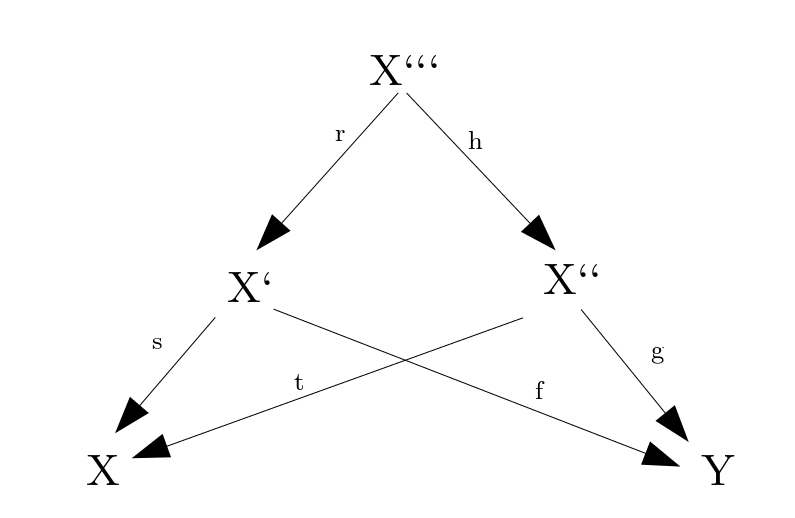
\includegraphics[scale=0.35]{roof-a_2.png} kommutiert.
    \item[iii) $Komposition \: von \: Morphismen \: durch \: (s,f), \: (t,g) \: ist \: Klasse \: von \: (st',gf')$:]
		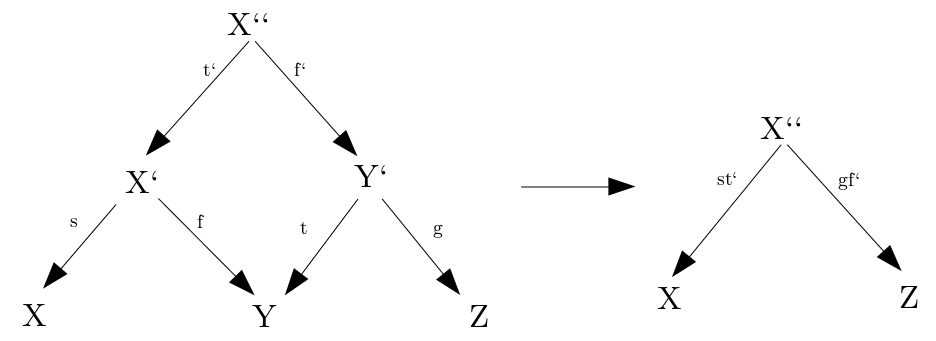
\includegraphics[scale=0.5]{roof-b.png}.
\end{description}

\subsection{Wann ist $B[S^{-1}]$ eine volle Unterkategorie von $C[S^{-1}]$}

Sei $B \subset C$ vollstaendige Unterkategorie, S Lokalisierungsklasse von C. Betrachte:
\begin{description}
    \item[i) $S_B = S \cap Mor(B) \: Lokalisierungssystem \: in \: B$]
    \item[ii) $\forall s \in S : X' \mapsto X \in Obj(B) \exists f : X'' \mapsto X'$:]
        \[sf \in S, \: X'' \in Ob(B)\]
    \item[iii) $wie \: ii) \: Pfeile \: umgekehrt$]   
\end{description}
Gilt i) und ii) oder iii), dann ist $B[S^{-1}] < C[S^{-1}]$ eine volle Unterkategorie und der kanonische Funktor
$k : B[S^{-1}] \mapsto C[S^{-1}]$ ist volltreu. 

\end{document}

 
\begin{thebibliography}{99}
\bib{gm}{book}{
   author={Gelfand, Sergei I.},
   author={Manin, Yuri I.},
   title={Methods of homological algebra},
   series={Springer Monographs in Mathematics},
   edition={2},
   publisher={Springer-Verlag, Berlin},
   date={2003},
   pages={xx+372},
   isbn={3-540-43583-2},
   review={\MR{1950475}},
   doi={10.1007/978-3-662-12492-5},
}

\bib{ml}{book}{
   author={Mac Lane, Saunders},
   title={Categories for the working mathematician},
   series={Graduate Texts in Mathematics},
   volume={5},
   edition={2},
   publisher={Springer-Verlag, New York},
   date={1998},
   pages={xii+314},
   isbn={0-387-98403-8},
   review={\MR{1712872}},
}

\end{thebibliography}
\end{document}
